\chapter{Implementation}
\label{chap:implementation}
\section{Preparations}
\subsection{Setting up a virtual machine}

For all developments within this thesis a virtual machine was used. This makes it easy to reproduce the environment within the labs at the TKRN group as well as having a portable development solution isolated from the rest of the computer's operating system. As the ROS version called \textit{Kinetic} is widely used within the set-ups around the robot, I will also develop the application using this version. This reduces the risk of incompatibility issues during development. ROS \textit{Kinetic} is available as packages for Ubuntu up to version 16.04\cite{ros:install}, which is why we install this version of Ubuntu within a new virtual machine. Enough virtual hard disk space and memory is assigned to the virtual machine (200GB HDD, 8 GB RAM) as well as 4 processing cores. This set-up should be sufficient for all purposes during this thesis. 

If the virtual machine shall run ROS nodes which have to be accessible by ROS nodes outside the machine itself (i.e. the Android tablet running the control application) the network interface of the virtual machine should be configured as a bridged network connection. This lets the network's DHCP (if present) assign the virtual machine it's own IP address reachable from the network. However, this was not possible within the university's network, as Oracle VirtualBox was not able to create a working bridged network adapter using the computer's Wi-Fi connection. During development within the lab another computer directly connected to the university network was used to run \textit{roscore}.

\subsection{Setting up ROS}

\subsubsection{Installing ROS}

Setting up ROS \textit{Kinetic} within a fresh Ubuntu 16.04 installation is fairly simple. First, the ROS apt\footnote{Aptitude is the package management system for Debian-based Linux distributions like Ubuntu}-repository has to be added to the packages sources file and the corresponding key has to be added to the key storage to enable downloading the packages. Once this is done, the package \textit{ros-kinetic-desktop-full} cann be installed which will download and install all available packages for ROS \textit{Kinetic}.

The commands to install ROS are denoted in Listing \ref{lst:ros:install}. After these commands have been executed in a terminal window ROS is readily installed.

\begin{minipage}{\linewidth}
	\begin{lstlisting}[caption={Commands for installing ROS\cite{ros:install}},label={lst:ros:install}]
	sudo sh -c 'echo "deb http://packages.ros.org/ros/ubuntu $(lsb_release -sc) main" > /etc/apt/sources.list.d/ros-latest.list'
	sudo apt-key adv --keyserver hkp://ha.pool.sks-keyservers.net:80 --recv-key 421C365BD9FF1F717815A3895523BAEEB01FA116
	sudo apt-get update
	sudo apt-get install ros-kinetic-desktop-full
	\end{lstlisting}
\end{minipage}

ROS is by default installed to \textit{/opt/ros/kinetic/}. To make use of all available command line tools provided by ROS it is important to load the file \textit{/opt/ros/kinetic/setup.bash} into the currently open (bash)-command-prompt. This is either temporarily done by issuing

\begin{lstlisting}[caption={Temporarily loading the ROS environment into bash}]
source /opt/ros/kinetic/setup.bash
\end{lstlisting}

or permanently by adding this line to the file \textit{$\sim$/.bashrc} by executing the following command:

\begin{lstlisting}[caption={Permamently installing the ROS environment into bash}]
echo "source /opt/ros/kinetic/setup.bash" >> ~/.bashrc
source ~/.bashrc
\end{lstlisting}

When this is done, ROS is completely set up on the development machine.

\subsubsection[Setting up catkin]{Setting up a catkin workspace\cite{ros:install:catkin}} 

\textit{Catkin\footnote{\url{http://wiki.ros.org/catkin}}} is a build system and workspace management utility provided with ROS. It supports developers to create, develop and build packages for ROS applications. To create a catkin workspace within the current user's home directory, issue the commands from Listing \ref{lst:ros:catkin} after setting up ROS and sourcing the \textit{setup.bash}-file.

\begin{minipage}{\linewidth}
	\begin{lstlisting}[caption={Setting up a catkin workspace},label=lst:ros:catkin]
mkdir -p ~/catkin_ws/src
cd ~/catkin_ws/
catkin_make

source devel/setup.bash
	\end{lstlisting}
\end{minipage}

ROS and catkin are now fully set up and can be used for further development.

\subsection{Installing Android Studio}

Android Studio is used as IDE during development of this thesis and should be installed according to the official documentation\footnote{\url{https://developer.android.com/studio/install.html}}. It is sensible to add the \textit{bin} directory in the installation path to the \textit{PATH} environment variable to make Android Studio accessible by just typing \textit{studio.sh} into a terminal window.

After Android Studio was installed successfully, it is important to select and install the correct Android SDK versions as the project will compile with the Android 7 compiler to work with Android 4. To do so, open The SDK Manager (\textit{Tools > Android > SDK Manager}) and select the SDKs according to Figure \ref{fig:android:sdk}. When this is done, Android Studio is set up to develop and compile the application.

\begin{figure}
	\caption{Needed Android SDKs\label{fig:android:sdk}}
	\begin{center}
		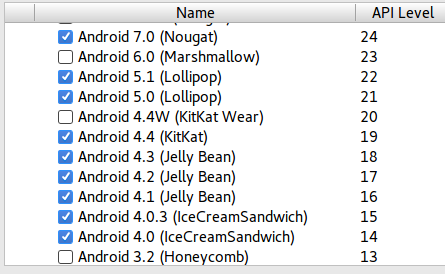
\includegraphics[scale=0.7]{assets/chpt_impl/sdks.PNG}
	\end{center}
\end{figure}

\subsection{Modifying and compiling rosandroid}
\label{impl:compiling_rosandroid}

Since the application developed in this thesis shall work on Android from versions beginning at 4.0.3 we have to modify the rosandroid code on one little detail to make everything work fine. In the created catkin workspace, go to the \textit{src} folder and clone the rosjava and rosandroid repositories there:
\begin{lstlisting}[caption={Cloning the rosandroid and rosjava repositories}]
git clone https://github.com/rosjava/rosjava_core.git
git clone https://github.com/rosjava/android_core.git
git clone https://github.com/rosjava/rosjava_messages.git
\end{lstlisting}

Then line 38 in the file
\begin{lstlisting}[numbers=none]
android_core/android_10/src/org/ros/android/RosActivity.java
\end{lstlisting}

has to be replaced by

\begin{lstlisting}[caption={Change to make to RosActivity.java},firstnumber=38,breaklines=true]
public abstract class RosActivity extends android.support.v7.app.AppCompatActivity {
\end{lstlisting}

This gives us the ability to use the already-built features in rosandroid like the automatically displayed activity to connect to a ROS master and built-in node handling even in older Android versions. When changes are made, issue a \textit{catkin\_make} command in the catkin workspace's root directory. \textit{Rosjava} and \textit{rosandroid} will then be built from source and deployed to a \textit{Maven}\footnote{Maven is a dependency and package management system for Java libraries.} repository from where the binaries will be loaded by Android Studio on compile time.

\section{User Interface}
\section{Software Architecture}
\section{Approaches}
\subsection{Grasp Synergies}
\subsection{Direct Finger Positioning}